\documentclass[a4paper,twoside,10pt]{book}
% PAGE DIMENSIONS
% FOR A5 without scaling
%\usepackage[inner=18mm, outer=10mm,top=20mm,headsep=10mm,bottom=10mm,paperwidth=148mm,paperheight=210mm]{geometry}
% FOR 17x24cm
\usepackage[inner=30mm, outer=20mm,top=24mm,headsep=10mm,bottom=20mm,paperwidth=170mm,paperheight=240mm]{geometry}
% FOR A4
%\usepackage[inner=50mm, outer=40mm,top=60mm,headsep=10mm,bottom=57mm,paperwidth=210mm,paperheight=297mm]{geometry}
%\usepackage[inner=8.5mm, outer=12.5mm,top=10mm,headsep=5mm,bottom=10mm,paperwidth=141mm,paperheight=200mm]{geometry}
%\usepackage[inner=30mm, outer=23mm,top=29mm,headsep=10mm,bottom=23mm,paperwidth=210mm,paperheight=297mm]{geometry}
% FOR A5
%\usepackage[inner=25mm, outer=17mm,top=8mm,headsep=8mm,bottom=17mm,paperwidth=148mm,paperheight=210mm,includehead]{geometry}
% TABLES: full-width using X{10cm} column
\usepackage{tabularx}
% DRAWINGS (for chapter title)
\usepackage{tikz}
% TYPOGRAPHY: 
\usepackage[protrusion=true,final,factor=1500]{microtype}

% SOME extra math symbols
\usepackage{amssymb}




% CAPTIONS of figures/table styling
\usepackage[font={stretch=1.1,small},labelfont=bf]{caption} % order matters: stretch, then size
%\usepackage[font={small,sf},labelfont=bf]{caption} % small sans-serif + bold

% FONT  SIZES
\usepackage{fix-cm} % FOR ANY font sizes, not predefined
\renewcommand\footnotesize{\fontsize{7pt}{7pt}\selectfont}
\renewcommand\small{\fontsize{6pt}{6pt}\selectfont}
\renewcommand\normalsize{\fontsize{9pt}{9pt}\selectfont}
\renewcommand\large{\fontsize{10pt}{10pt}\selectfont}
\renewcommand\Large{\fontsize{11pt}{11pt}\selectfont}
\renewcommand\Huge{\fontsize{24pt}{24pt}\selectfont}

% LINE spacing
\renewcommand{\baselinestretch}{1.25}

% FONTS for LaTeX/XeLaTeX
\usepackage{ifxetex}
\ifxetex
			\usepackage{mathspec}
			\usepackage{polyglossia}
			\setdefaultlanguage[variant=uk]{english}
			\defaultfontfeatures{Ligatures=TeX} % To support LaTeX quoting style
			\setmainfont{Minion Pro} 
			\setsansfont{Myriad Pro}
			\setmathsfont(Digits,Greek,Latin)[Numbers={Proportional}]{Minion Pro}
			\setmathrm{Minion Pro}
			\usepackage[italic]{mathastext}
			%\setmainfont[BoldFont={SwiftNeueLTW01-Bold},ItalicFont={SwiftNeueLTW01-Italic}]{SwiftNeueLTW01} 
			%\setsansfont{UniversLTW01-55Roman}
\else
			%\usepackage[T1]{fontenc}
			%\usepackage[utf8]{inputenc}
			\usepackage[english]{babel}
			%\usepackage{fouriernc} % UTOPIA + FOURIER
			%\usepackage{mathpple} % palatino
			%\usepackage[sc]{mathpazo}
			\usepackage[charter]{mathdesign} %utopia, garamond
			\usepackage[scaled]{helvet}
			%\usepackage{newtxtt}
			\def\ttdefault{cmvtt}
			%\usepackage[light]{roboto}
			%\renewcommand{\sfdefault}{ua1}
\fi

\usepackage{hyperref}
% HEADER/FOOTER
\usepackage{fancyhdr}
\renewcommand{\headrulewidth}{0pt}
\renewcommand{\footrulewidth}{0pt}
\fancyhf{}
\makeatletter
	\let\ps@plain\ps@empty
\makeatother
% PLAIN: for first page of chapter
\fancypagestyle{plain}{
	\renewcommand{\headrulewidth}{0pt}
	\fancyhf{}
	\fancyhead[RO]{
		\makebox[2cm][l]{
			\makebox[4cm][c]{\normalsize
				\hskip0.25em\phantom{\thepage}\phantom{XX}~~$\left|\vphantom{\int_a^b}\right.$~~\thepage\phantom{XX}
			}
		}
	}
	\fancyhead[LE]{
		\makebox[2cm][r]{
			\makebox[4cm][c]{\normalsize
				\hskip0.45em\phantom{XX}\thepage~~$\left|\vphantom{\int_a^b}\right.$~~\phantom{XX}\phantom{\thepage}
			}
		}
	}
}
% REGULAR pages
\fancyhead[RO]{
	\makebox[2cm][l]{
		\makebox[4cm][c]{\normalsize
			\hskip0.25em\phantom{\thepage}\nouppercase\rightmark~~$\left|\vphantom{\int_a^b}\right.$~~\thepage\phantom{\nouppercase\rightmark}
		}
	}
}
\fancyhead[LE]{
	\makebox[2cm][r]{
		\makebox[4cm][c]{\normalsize
			\hskip0.45em\phantom{\nouppercase\leftmark}\thepage~~$\left|\vphantom{\int_a^b}\right.$~~\nouppercase\leftmark\phantom{\thepage}
		}
	}
}

% MARGIN labels, except chapter=0 (intro; conclusion; bibliography etc.)
% AND \setcouter{chapter}{0} has to be set explicitely in required chapters
\fancyfoot[RO]{
	\ifnum\value{chapter}>0
	\begin{tikzpicture}[remember picture, overlay]
	\node[rounded corners=2mm,inner sep=3mm,anchor=north east,black,fill=black!15,draw=black!75] at ([xshift=2mm,yshift=-\arabic{chapter}*1.3cm-1.1cm]current page.north east) {\fontsize{1cm}{1cm}\selectfont\thechapter};
	\end{tikzpicture}
	\fi
}
\fancyfoot[LE]{
	\ifnum\value{chapter}>0
	\begin{tikzpicture}[remember picture, overlay]
	\node[rounded corners=2mm,inner sep=3mm,anchor=north west,black,fill=black!15,draw=black!75] at ([xshift=-2mm,yshift=-\arabic{chapter}*1.3cm-1.1cm]current page.north west) {\fontsize{1cm}{1cm}\selectfont\thechapter};
	\end{tikzpicture}
	\fi
}



\pagestyle{fancy}
% HEADER contents - chapter name and section name
%\renewcommand{\chaptermark}[1]{\markboth{\thechapter.\, #1}{}}
\renewcommand{\chaptermark}[1]{\markboth{#1}{}}
\renewcommand{\sectionmark}[1]{\markright{\thesection.\, #1}}


% FLOATING objects
\usepackage{float}
% PICTURES
\usepackage{graphicx}
% NOT USED
\usepackage{setspace}

% SPACINGS in lists
\usepackage{enumitem}
% VERICAL: topsep partopsep parsep itemsep
% HORIZONTAL: leftmargin rightmargin listparindent labelwidth labelsep itemindent
% GLOBAL: \setlist[enumerate]{labelsep=*, leftmargin=1.5pc}
%\setlist{noitemsep}
\setlist{nosep}




% TABLES: nicer rulers
% AND nicer spacing between lines in tables
\usepackage{booktabs}
\renewcommand{\arraystretch}{1.2}


% TITLES styling
\usepackage[toctitles,explicit,raggedright]{titlesec}
\newcommand*\chapterlabel{}
% CHAPTER in frontmatter|backmatter
\titleformat{name=\chapter,numberless}[display]
	{\normalfont\rmfamily\Huge\bfseries}{}{1ex}
	{\flushright{\chapterlabel#1}}
% CHAPTER in mainmatter
\titleformat{\chapter}
{\gdef\chapterlabel{}\normalfont\rmfamily\Huge\bfseries}
{\gdef\chapterlabel{}}{-10em}
{
	\flushright{
		\begin{tikzpicture}
			%\draw[help lines,step=5mm] (0,-3) grid (-\linewidth,3);
			\node[black!50,anchor=east,inner sep=0mm] (a) at (0,0) {\fontsize{7cm}{8cm}\selectfont\thechapter};
			\begin{scope}[cm={1,0,-0.6,0.15,(0,0)}].
					\node[transform shape,black!30,anchor=south,inner sep=0mm] at (a.south) {\fontsize{7cm}{8cm}\selectfont{}\thechapter};
					%\node[transform shape,black!30,anchor=south east,inner sep=0mm] at (a.south) {\fontsize{3cm}{8cm}\selectfont{}\chaptername};
			\end{scope}
			\node[black!50,anchor=east,inner sep=0mm] (a) at (0,0) {\fontsize{7cm}{8cm}\selectfont\thechapter};
			\node[black!35,anchor=east,inner sep=0.20mm,scale=0.98] at (0,0) {\fontsize{7cm}{8cm}\selectfont\thechapter};
			\node[black!20,anchor=east,inner sep=0.40mm,scale=0.96] at (0,0) {\fontsize{7cm}{8cm}\selectfont\thechapter};
			%\node[black!20,scale=0.97] at (a) {\fontsize{6cm}{8cm}\selectfont\thechapter};
			%\node[anchor=east,black!45] at (0,-1) {\resizebox{\linewidth}{!}{\chaptername}};
			%\node[anchor=north east,inner sep=0mm] at (a.north east) {\parbox{\linewidth}{\raggedleft\chapterlabel#1}};
			\node[anchor=east,inner sep=0mm] at (0,0) {\parbox{\linewidth}{\raggedleft\chapterlabel#1}};
		\end{tikzpicture}
		%\chapterlabel#1
	}
}
% SPACING: chapter by default uses \@makechapterhead with extra spacing before and after the chapter title
\titlespacing*{\chapter}{0pt}{-25pt}{30pt}

%\titleformat{\section}[block]{\Large}{\bfseries\thesection.\,\,#1}{1em}{}
%\titleformat{\subsection}[block]{\large}{\bfseries\thesubsection.\,\,#1}{1em}{}
%\titleformat{\subsection}{\no}{\itshape\thesubsection.\,#1}{1em}{}


% GREEK letters in section/chapter titles AND in PDF bookmarks
%\usepackage[artemisia]{textgreek}




\usepackage{listings}
\definecolor{mygreen}{rgb}{0,0.6,0}
\definecolor{mygray}{rgb}{0.5,0.5,0.5}
\definecolor{mymauve}{rgb}{0.58,0,0.82}
\usepackage{amsmath}
\usepackage{pgfplots}

\lstset{ 
	backgroundcolor=\color{white},   % choose the background color; you must add \usepackage{color} or \usepackage{xcolor}; should come as last argument
	basicstyle=\small\ttfamily,
	belowcaptionskip=0em,        % the size of the fonts that are used for the code
	belowskip=-2em,
	breakatwhitespace=false,         % sets if automatic breaks should only happen at whitespace
	breaklines=true,                 % sets automatic line breaking
	captionpos=b,                    % sets the caption-position to bottom
	commentstyle=\color{mygreen},    % comment style
	deletekeywords={...},            % if you want to delete keywords from the given language
	escapeinside={\%*}{*)},          % if you want to add LaTeX within your code
	extendedchars=true,              % lets you use non-ASCII characters; for 8-bits encodings only, does not work with UTF-8
	frame=single,	                   % adds a frame around the code
	keepspaces=true,                 % keeps spaces in text, useful for keeping indentation of code (possibly needs columns=flexible)
	keywordstyle=\color{blue},       % keyword style
	language=Python,                 % the language of the code
	morekeywords={*,...},            % if you want to add more keywords to the set
	numbers=none,                    % where to put the line-numbers; possible values are (none, left, right)
	numbersep=5pt,                   % how far the line-numbers are from the code
	numberstyle=\tiny\color{mygray}, % the style that is used for the line-numbers
	rulecolor=\color{black},         % if not set, the frame-color may be changed on line-breaks within not-black text (e.g. comments (green here))
	showspaces=false,                % show spaces everywhere adding particular underscores; it overrides 'showstringspaces'
	showstringspaces=false,          % underline spaces within strings only
	showtabs=false,                  % show tabs within strings adding particular underscores
	stepnumber=2,                    % the step between two line-numbers. If it's 1, each line will be numbered
	stringstyle=\color{mymauve},     % string literal style
	tabsize=2,	                   % sets default tabsize to 2 spaces
	title=\lstname 			          % show the filename of files included with \lstinputlisting; also try caption instead of title
}
\def\inline{\lstinline[basicstyle=\ttfamily,keywordstyle={}]} %https://tex.stackexchange.com/questions/44702/can-you-change-lstinline-without-changing-the-global-lstset

% https://tex.stackexchange.com/questions/31085/is-there-a-standard-way-to-title-a-list-of-bullets
% name is purpose
\newenvironment{exercize}[1]{%
\vspace{0.2em}\noindent{\Large\textbf{#1}}
	\begin{itemize}}
	{\end{itemize}}
\begin{document}
\chapter{Improving the way neural networks learn}
When a golf player is first learning to play golf, they usually spend most of their time developing a basic swing. Only gradually do they develop other shots, learning to chip, draw and fade the ball, building on and modifying their basic swing. In a similar way, up to now we've focused on understanding the backpropagation algorithm. It's our "basic swing", the foundation for learning in most work on neural networks. In this chapter I explain a suite of techniques which can be used to improve on our vanilla implementation of backpropagation, and so improve the way our networks learn.

The techniques we'll develop in this chapter include: a better choice of cost function, known as the cross-entropy cost function; four so-called ``regularization'' methods (L1 and L2 regularization, dropout, and artificial expansion of the training data), which make our networks better at generalizing beyond the training data; a better method for initializing the weights in the network; and a set of heuristics to help choose good hyper-parameters for the network. I'll also overview several other techniques in less depth. The discussions are largely independent of one another, and so you may jump ahead if you wish. We'll also implement many of the techniques in running code, and use them to improve the results obtained on the handwriting classification problem studied in Chapter 1.

Of course, we're only covering a few of the many, many techniques which have been developed for use in neural nets. The philosophy is that the best entree to the plethora of available techniques is in-depth study of a few of the most important. Mastering those important techniques is not just useful in its own right, but will also deepen your understanding of what problems can arise when you use neural networks. That will leave you well prepared to quickly pick up other techniques, as you need them.

\section{The cross-entropy cost function}
Most of us find it unpleasant to be wrong. Soon after beginning to learn the piano I gave my first performance before an audience. I was nervous, and began playing the piece an octave too low. I got confused, and couldn't continue until someone pointed out my error. I was very embarrassed. Yet while unpleasant, we also learn quickly when we're decisively wrong. You can bet that the next time I played before an audience I played in the correct octave! By contrast, we learn more slowly when our errors are less well-defined.

Ideally, we hope and expect that our neural networks will learn fast from their errors. Is this what happens in practice? To answer this question, let's look at a toy example. The example involves a neuron with just one input:

\begin{center}
	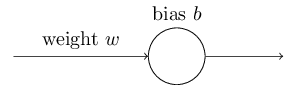
\includegraphics[width=0.5\linewidth]{figures/ch3/tikz28}
\end{center}
We'll train this neuron to do something ridiculously easy: take the input 1 to the output 0. Of course, this is such a trivial task that we could easily figure out an appropriate weight and bias by hand, without using a learning algorithm. However, it turns out to be illuminating to use gradient descent to attempt to learn a weight and bias. So let's take a look at how the neuron learns.

To make things definite, I'll pick the initial weight to be 0.6 and the initial bias to be 0.9. These are generic choices used as a place to begin learning, I wasn't picking them to be special in any way. The initial output from the neuron is 0.82, so quite a bit of learning will be needed before our neuron gets near the desired output, 0.0. Click on "Run" in the bottom right corner below to see how the neuron learns an output much closer to 0.0. Note that this isn't a pre-recorded animation, your browser is actually computing the gradient, then using the gradient to update the weight and bias, and displaying the result. The learning rate is $\eta$=0.15, which turns out to be slow enough that we can follow what's happening, but fast enough that we can get substantial learning in just a few seconds. The cost is the quadratic cost function, $C$, introduced back in Chapter 1. I'll remind you of the exact form of the cost function shortly, so there's no need to go and dig up the definition. Note that you can run the animation multiple times by clicking on ``Run'' again.
\begin{lstlisting}

ANIMATION
\end{lstlisting}
As you can see, the neuron rapidly learns a weight and bias that drives down the cost, and gives an output from the neuron of about 0.09. That's not quite the desired output, 0.0, but it is pretty good. Suppose, however, that we instead choose both the starting weight and the starting bias to be 2.0. In this case the initial output is 0.98, which is very badly wrong. Let's look at how the neuron learns to output 0 in this case. Click on "Run" again:
\begin{lstlisting}

ANIMATION
\end{lstlisting}
Although this example uses the same learning rate ($\eta=0.15$), we can see that learning starts out much more slowly. Indeed, for the first 150 or so learning epochs, the weights and biases don't change much at all. Then the learning kicks in and, much as in our first example, the neuron's output rapidly moves closer to 0.0.

This behaviour is strange when contrasted to human learning. As I said at the beginning of this section, we often learn fastest when we're badly wrong about something. But we've just seen that our artificial neuron has a lot of difficulty learning when it's badly wrong - far more difficulty than when it's just a little wrong. What's more, it turns out that this behaviour occurs not just in this toy model, but in more general networks. Why is learning so slow? And can we find a way of avoiding this slowdown?

To understand the origin of the problem, consider that our neuron learns by changing the weight and bias at a rate determined by the partial derivatives of the cost function, $\partial{}C/\partial{}w$ and $\partial{}C/\partial{}b$. So saying ``learning is slow'' is really the same as saying that those partial derivatives are small. The challenge is to understand why they are small. To understand that, let's compute the partial derivatives. Recall that we're using the quadratic cost function, which, from Equation \ref{eq:6}, is given by
\begin{equation}
C = \frac{(y-a)^2}2,\label{eq:54}
\end{equation}
where $a$ is the neuron's output when the training input $x=1$ is used, and $y=0$ is the corresponding desired output. To write this more explicitly in terms of the weight and bias, recall that $a=\sigma{}(z)$, where $z=wx+b$. Using the chain rule to differentiate with respect to the weight and bias we get
\begin{eqnarray} 
\frac{\partial C}{\partial w} & = & (a-y)\sigma'(z) x = a \sigma'(z) \label{eq:55}\\
\frac{\partial C}{\partial b} & = & (a-y)\sigma'(z) = a \sigma'(z),
\label{eq:56}
\end{eqnarray}
where I have substituted $x=1$ and $y=0$. To understand the behaviour of these expressions, let's look more closely at the $\sigma{}'(z)$ term on the right-hand side. Recall the shape of the $\sigma{}$ function:

\begin{tikzpicture}[scale=0.75]
\begin{axis}[title={Sigmoid function}]
\addplot[blue,domain=-5:5,samples=81]{1/(1+exp(-x)};
\end{axis}
\end{tikzpicture}

We can see from this graph that when the neuron's output is close to 1, the curve gets very flat, and so $\sigma{}'(z)$ gets very small. Equations \ref{eq:55} and \ref{eq:56} then tell us that $\partial{}C/\partial{}w$ and $\partial{}C/\partial{}b$ get very small. This is the origin of the learning slowdown. What's more, as we shall see a little later, the learning slowdown occurs for essentially the same reason in more general neural networks, not just the toy example we've been playing with.
\section{Introducing the cross-entropy cost function}

\end{document}
